\documentclass{article}



\usepackage{arxiv}

\usepackage[utf8]{inputenc} % allow utf-8 input
\usepackage[T1]{fontenc}    % use 8-bit T1 fonts
\usepackage{hyperref}       % hyperlinks
\usepackage{url}            % simple URL typesetting
\usepackage{booktabs}       % professional-quality tables
\usepackage{amsfonts}       % blackboard math symbols
\usepackage{amsmath}
\usepackage{xcolor}
\usepackage{nicefrac}       % compact symbols for 1/2, etc.
\usepackage{microtype}      % microtypography
\usepackage{lipsum}		% Can be removed after putting your text content
\usepackage{graphicx}
\usepackage{natbib}
\usepackage{doi}





\title{GP-KAN: Gaussian Process Kolmogorov-Arnold Networks}

%\date{September 9, 1985}	% Here you can change the date presented in the paper title
%\date{} 					% Or removing it

\author{
	{\hspace{1mm}Andrew S. Chen}\thanks{Currently employed at Arm, UK} \\
	University of Cambridge\\
	sc2178@cantab.ac.uk
}

% Uncomment to remove the date
%\date{}

% Uncomment to override  the `A preprint' in the header
\renewcommand{\headeright}{}
\renewcommand{\undertitle}{}
% \renewcommand{\shorttitle}{\textit{arXiv} Template}

%%% Add PDF metadata to help others organize their library
%%% Once the PDF is generated, you can check the metadata with
%%% $ pdfinfo template.pdf
\hypersetup{
pdftitle={A template for the arxiv style},
pdfsubject={q-bio.NC, q-bio.QM},
pdfauthor={David S.~Hippocampus, Elias D.~Striatum},
pdfkeywords={First keyword, Second keyword, More},
}

\begin{document}
\maketitle

\begin{abstract}
	TODO
\end{abstract}


% keywords can be removed
\keywords{Gaussian Process \and Kolmogorov-Arnold Networks}


\section{Introduction}
TODO


\section{Background}
\subsection{Kolmogorov-Arnold Networks}
Kolmogorov-Arnold Networks (KANs) \cite{liu2024kan} are class of networks inspired by the Kolmogorov-Arnold Representation Theorem \cite{AndreyKolmogorov,VladimirArnold} which establishes that any bounded multivariate continuous function $f$ can be rewritten as a composition of univariate functions $\phi$ and the binary operator of addition. The original formulation of the theorem examines a composition of 2 layers:
\begin{equation}
    f(x_1, x_2, ... x_n) = \sum_{q=1}^{2n}\phi_{q,n+1}\left(\sum_{p=1}^{n}\phi_{q,p}(x_p)\right)
    \label{eq:Kolmogorov-Arnold-Theorem}
\end{equation}
but provides no guarentees on the nature of $\phi$, which can be non-smooth and possess characteristics that hinder learning them. KANs generalizes the concept to arbitary depths and widths, such that $\phi$ becomes learnable via traditional machine learning tools such as back propagation. The KANs proposed \cite{liu2024kan} uses B-spline to approximate $\phi$, and has shown that given the appropriate choices of basis functions, KAN is able to recover the exact symbolic formulation of various multivariate functions, and at times discover alternative formulations. Further work \cite{li2024kolmogorovarnold} expanding on the use of Radial Basis Functions (RBF) have been successful in applying KANs to machine learning problems such as MNIST image classification \cite{MNIST}. It becomes clear that the choice of basis functions greatly impacts the modelling capabilities of KANs.

\subsection{Gaussian Process}
Gaussian Process (GP) \cite{GaussianProcess} describes the probability distribution over functions by treating functions as a collection of Random Variables (r.v.) where any finite subset has a joint Gaussian Distribution. A GP is fully specified by its mean function $m(\cdot)$ and covariance function $k(\cdot, \cdot)$.
\begin{equation}
    \begin{aligned}
        f                                    & \sim\mathcal{GP}(m,k)
        \\
        \text{where} \quad m(x) & =\mathbb{E} [f(x)]
        \\
        k(x,x')    & =\text{Covar}[f(x), f(x')]
    \end{aligned}
    \label{eq:GP_def}
\end{equation}
Given a set of known noisy function values $\boldsymbol{h}$ at locations $\boldsymbol{z}$, GP prediction at a new location $x$ follows Equation \ref{eq:GP_pred}. In GP regression, $\boldsymbol{h}, \boldsymbol{z}$ corresponds to known data labels and inputs, with label noise $\sigma_n^2$ and the training objective of maximising their likelihood (or equivalently the log-likelihood). A key drawback of Gaussian Process is the \textbf{curse of dimensionality}, due to the $\mathcal{O}(n^3)$ complexity of inverting $K_{hh}$ in Equation \ref{eq:GP_pred} for $n$ data points and the need for large $\boldsymbol{h}, \boldsymbol{z}$ to map the input space for high-dimensional inputs.
\begin{equation}
    \begin{aligned}
        p(f|\boldsymbol{h},\boldsymbol{z},x)     & =\mathcal{N}(\mu, \Sigma)           \\
        \text{where}\quad\quad\mu & =m(x) + \boldsymbol{k}_{xh}(K_{hh}+\sigma_n^2 I)^{-1}\boldsymbol{h} \\
        \Sigma                    & =k(x, x)-\boldsymbol{k}_{xh}(K_{hh}+\sigma_n^2 I)^{-1}\boldsymbol{k}_{hx}        \\
        \boldsymbol{k}_{xh}^T                  & =\boldsymbol{k}_{hx}=\begin{bmatrix}
                                                k(z_1, x) \\
                                                k(z_2, x) \\
                                                \vdots
                                            \end{bmatrix}                  \\
        K_{hh}                    & =\begin{bmatrix}
                                         k(z_1,z_1) & k(z_1, z_2) & \hdots \\
                                         k(z_2,z_1) &             &        \\
                                         \vdots     &             &
                                     \end{bmatrix}
    \end{aligned}
    \label{eq:GP_pred}
\end{equation}

\section{GP-KAN}
GPs and KANs have the potential to be natural complements. KANs only considers the usage of univariate functions $\phi$, avoiding GPs' \textbf{curse of dimensionality}. For a given input $x$, and known data $\boldsymbol{h}, \boldsymbol{z}$, the predictive GP defines the distribution of an output Gaussian r.v. $p(f|\boldsymbol{h},\boldsymbol{z},x)$, and the set of Gaussian r.v. is closed under the binary operation of addition, the only multivariate operator in KANs. On the other hand, KANs rely on good choices of basis functions for $\phi$, and it can be shown that the \textit{squared exponential} covariance function (Equation \ref{eq:covar_se}) corresponds to a Bayesian Linear Regression Model of infinite number of RBFs \cite[Sect 4.3 \& Eq 4.13]{GaussianProcess}.
\begin{equation}
    k(x,x')=s^2\exp\left(-\frac{(x-x')^2}{2l^2}\right)=s^2l\sqrt{2\pi}\mathcal{N}(x|x',l^2)
    \label{eq:covar_se}
\end{equation}
Almost immediately, however, one runs into the problem that for an input Gaussian Distribution $p(x)$, the output distribution $p(f|\boldsymbol{h},\boldsymbol{z})=\int p(f|\boldsymbol{h},\boldsymbol{z},x)p(x)dx$ is often intractable and not Gaussian \cite{deepGP, GPLVM}. This underlies an obstacle in the usage of multi-layer GP networks whilst trying to maintain a fully Bayesian treatment. One solution is Monte-Carlo estimation, which suffers from steep computational cost and poor estimation in high-dimensional problemsets. Other approaches \cite{deepGP} rely on variational methods to provide a tractable strict lower bound to the objective function, the training data likelihood in this case.

The following approach revolves around effort to maintain the following:
\begin{enumerate}
    \item All model intermediate elements, whose distribution depends on the model's input data's distribution, are Gaussian r.v.
    \item All model intermediate elements are independent
    \item All GPs within the model are univariate GPs
\end{enumerate}
Item 1 and 3 helps to simplify analysis and produce a fully tractable exact objective function, while Item 2 allows one to avoid tracking covariance between intermediate elements of the model, keeping the computational complexity to $O(n)$ for $n$ intermediate elements.
\subsection{Single GP neuron}
Consider the following r.v. $y$
\begin{equation}
	y=f\ast p(x)=\int f p(x)dx,\text{ for }p(x)=\mathcal{N}(x|\mu_x,\sigma_x^2), f\sim\mathcal{GP}(m(\cdot),k(\cdot,\cdot)|\boldsymbol{h},\boldsymbol{z})
    \label{eq:reformulation}
\end{equation}
where $\ast$ is the \textit{convolution} operation for functions, and $f$ is drawn from the GP conditioned on $\boldsymbol{h},\boldsymbol{z}$. Equation \ref{eq:reformulation} can be seen as a summation over Gaussian r.v. composing $f$, each scaled by $p(x)$, and so $y$ is also a Gaussian r.v.. With Equation \ref{eq:covar_se} as the choice of covariance function, and a mean function $m(x)=0$, $y$'s distribution has an analytical form. Refer to Appendix \ref{apd:singleGPNeuron} for the derivation and interpretation of Equation \ref{eq:reformulation} and \ref{eq:gpneuron}.
\begin{equation}
    \begin{aligned}
        y&\sim\mathcal{N}(\mu_y, \sigma_y^2) \\
        \mu_y&=\sqrt{2\pi}s^2l\boldsymbol{q}_{xh}(K_{hh}+\sigma_n^2 I)^{-1}\boldsymbol{h} \\
        \sigma_y^2&=\frac{s^2l}{\sqrt{l^2+2\sigma_x^2}} - 2\pi s^4 l^2 \boldsymbol{q}_{xh}(K_{hh}+\sigma_n^2 I)^{-1}\boldsymbol{q}_{hx} \\
        \text{where }\boldsymbol{q}_{xh}^T&=\boldsymbol{q}_{hx}=\begin{bmatrix}
            \mathcal{N}(z_1|\mu_x,\sigma_x^2+l^2) \\
            \mathcal{N}(z_2|\mu_x,\sigma_x^2+l^2) \\
            \vdots
        \end{bmatrix}
        \label{eq:gpneuron}
    \end{aligned}
\end{equation}
This forms the foundation of a single GP neuron. Unlike the traditional Neuron \cite{ANN} which takes an input value and produces an output value, the GP neuron takes as input the distribution of a Gaussian r.v., and outputs the distribution of a Gaussian r.v.. The trainable parameters of the GP neuron would be the GP reference points $\boldsymbol{h}, \boldsymbol{z}$, reference noise $\sigma_n^2$ and the \textit{squared exponential} covariance function parameters $l, s$.

\subsection{Fully-Connected GP Layer (FCGP)}
The GP neuron equivalent of a Fully-Connected layer can defined, by using the binary operator of addition, as used in Kolmogorov-Arnold Representation Theorem. $\ast$ represents the \textit{convolution} for functions.
\begin{equation}
    y_i = \sum_{j=1}^{n} f_{i,j} \ast \mathcal{N}_j, \quad f_{i,j}\sim\mathcal{GP}_{i,j}
\end{equation}
TODO: appendix for efficient implementation using standard ML ops

TODO: evaluation on the nature of cross-correlation in the outputs -- there is none
\begin{equation}
    \begin{bmatrix}
        y_1 \\ y_2 \\ \vdots \\ y_m
    \end{bmatrix} =
    \begin{bmatrix}
        f_{1,1} & f_{1,2} & \hdots & f_{1,n} \\
        f_{2,1} & f_{2,2} & \hdots \\
        \vdots \\
        f_{m,1}
    \end{bmatrix}\ast
    \begin{bmatrix}
        p(x_1) \\ p(x_2) \\ \vdots \\ p(x_n)
    \end{bmatrix},\quad p(x_i) = \mathcal{N}_i = \mathcal{N}(\mu_{x,i},\sigma_{x,i}^2)
\end{equation}

\subsection{Convolutional GP Layer (ConvGP)}
Convolutional Neural Networks \cite{CNN} are a class of Neural Networks that are very effective at capturing translation-invariant features of input data, and are central to solving image-related problems. One can define the GP neuron equivalent by transforming an image of pixels (every pixel captures the distribution of a Gaussian r.v. instead of a singular value) into vectors via the im2col routine \cite{im2col_first,im2col_phdthesis}, passing it as a batch of input vectors through FCGP to output a batch of output vectors, and transforming via col2im (inverse im2col) back into an image (Figure \ref{fig:Convolutional_GP}). Since the same FCGP layer is used to process each input vector representing the moving convolution kernel, and produce an output vector representing the elements across channels in a single pixel of the output image, one has to note that every output pixel is considered \textit{conditionally independent} given the FCGP's internal GP reference points.

In practice, it is noted that using 2 FCGP layers in series within a single ConvGP layer can improve modelling capabilities. This points one back to the Kolmogorov-Arnold Representation Theorem (Equation \ref{eq:Kolmogorov-Arnold-Theorem}), whose equivalence of any multivariate function to composition of univariate functions over the binary operation of addition require the composition to have 2 layers.

\begin{figure}[t]
    \centering
    
\includegraphics[width=0.9\columnwidth]{Convolutional_GP.pdf}
    \caption{Convolutional GP (ConvGP) Layer}
    \label{fig:Convolutional_GP}
\end{figure}

\subsection{Activation Functions}
With the replacement of single values with distributions of Gaussian r.v. in the network, the selection of activation functions is now more restrictive if one aims to preserve the Gaussian-nature of the distributions. Linear functions such as AveragePool \cite{poolingmethods} are useable, since linear operations over Gaussian r.v. produces Gaussian r.v., although special care should be taken in the case of AveragePool to avoid overlapping pooling windows, which introduces cross-correlation between output Gaussian r.v. elements. Non-linear functions such as Sigmoid and Softmax are not suitable, since they break the Gaussian nature of the distributions, and in the case of Softmax, introduces cross-correlation across the Gaussian r.v..

Instead, the FCGP layer (or a series of them) is relied on to learn any required activation function that considers the relationship between elements in a vector of Gaussian r.v., without introducing cross-correlation in the output. This builds on the idea of learnable activation functions \cite{learnableActivations}, except that one is using infinite RBFs.

\subsubsection{Normalizing Map}
It is beneficial to bound the distributions (mean and variance) of Gaussian r.v. in the graph, to avoid exploding gradients in back propagation during training. However, the set of Gaussian r.v. is only closed under linear operations, which do not serve well the purpose of bounding the distribution parameter values.

Given $\mathcal{G}$ denoting the set of unbounded Gaussian r.v. whose mean $\mu\in(-\infty,\infty) $ and variance $\sigma^2\in[0,\infty)$, and $\mathcal{G}'$ denoting the set of bounded Gaussian r.v. whose mean $\mu\in[a,b]$ and variance $\sigma^2\in[0,c]$ and $a,b,c$ are finite, a bijective map $\gamma: \mathcal{G} \rightarrow \mathcal{G}'$ can be chosen, such as the following:
\begin{equation}
    \begin{aligned}
        \text{for }&x\in\mathcal{G},\quad x\sim\mathcal{N}(\mu_x,\sigma_x^2) \\
        \text{define }&y\sim\mathcal{N}(\mu_y, \sigma_y^2) \\
        \text{where }&\mu_y = \text{tanh}(\mu_x) \\
                     &\sigma_y^2 = \text{sigmoid}(\sigma_x^2 - \mu_x^2) \\
        \text{then }&y\in\mathcal{G}' \text{ where }a=-1,\space b=c=1
    \end{aligned}
    \label{eq:normalizeMap}
\end{equation}
Such a bijective map has the below properties, avoiding the problem of exploding gradients and stabilising the training process.
\begin{enumerate}
    \item for $\mu_x\rightarrow\pm\infty$, one gets $\mu_y\rightarrow\pm 1$ and $\sigma_y^2\rightarrow 0$
    \item for $\sigma_x^2\rightarrow\infty$, one gets $\sigma_y^2\rightarrow 1$
\end{enumerate}

\section{Experiments}
lll
\subsection{Toy Data}


\subsection{Image Classication - MNIST}
A simple model (Figure \ref{fig:MNIST_model}) is used to train on the MNIST dataset \cite{MNIST}, and

\begin{table}
    \caption{Sample table title}
     \centering
     \begin{tabular}{lll}
       \toprule
       \multicolumn{3}{c}{MNIST}                                 \\
       \cmidrule(r){1-3}
       Model     & Accuracy & \#Params     \\
       \midrule
       ConvolutionalKAN\cite{ConvolutionalKAN} & 98.9\% & 95K  \\
       \bottomrule
     \end{tabular}
     \label{tab:table}
\end{table}

\begin{figure}[t]
    \centering
    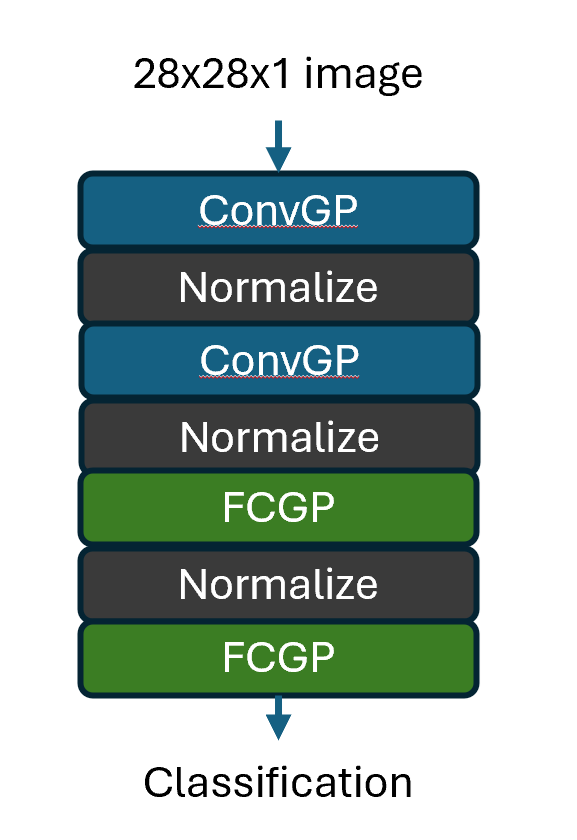
\includegraphics[width=0.9\columnwidth]{MNIST_model.png}
    \caption{MNIST classification for different models. Each model follows the above model structure, with different number of training parameters by changing kernel, channel and stride sizes. Every individual GP neuron has 10 trainable reference points. The models are trained on 55k training set and 5k validation set.}
    \label{fig:MNIST_model}
\end{figure}


\bibliographystyle{unsrt}
\bibliography{references}

\newpage
\appendix

\section{Single GP Neuron Derivation}
\label{apd:singleGPNeuron}
\subsection{Derivation for Equation \ref{eq:gpneuron}}

First note the following identity:
\begin{equation}
    \int\mathcal{N}(\boldsymbol{y}|W\boldsymbol{x}+\boldsymbol{b},\Sigma_2)\mathcal{N}(\boldsymbol{x}|\mu,\Sigma_1)d\boldsymbol{x}=\mathcal{N}(\boldsymbol{y}|W\mu+\boldsymbol{b},W\Sigma_1W^T+\Sigma_2)
    \label{eq:int_gaussian}
\end{equation}
Equation \ref{eq:int_gaussian} can be proven by considering Gaussian random variable $\Tilde{\boldsymbol{x}}\sim\mathcal{N}(\boldsymbol{x}|\mu,\Sigma_1)$ and $\Tilde{\boldsymbol{e}}\sim\mathcal{N}(\boldsymbol{e}|\boldsymbol{b},\Sigma_2)$. Then the Gaussian random variable $\Tilde{\boldsymbol{y}}=(W\Tilde{\boldsymbol{x}}+\Tilde{\boldsymbol{e}})\sim\mathcal{N}(\boldsymbol{y}|W\mu+\boldsymbol{b},W\Sigma_1W^T+\Sigma_2)$. Marginalizing the distribution for $\Tilde{\boldsymbol{y}}$ gives $p(\boldsymbol{y})=\int p(\boldsymbol{y}|\boldsymbol{x})p(\boldsymbol{x})d\boldsymbol{x}$, where we note that $p(\boldsymbol{x})=\mathcal{N}(\boldsymbol{x}|\mu,\Sigma_1)$ and $p(\boldsymbol{y}|\boldsymbol{x})=\mathcal{N}(\boldsymbol{y}|W\boldsymbol{x}+\boldsymbol{b},\Sigma_2)$, thus giving Equation \ref{eq:int_gaussian}. This Equation is also found in a more general form \cite{MatrixCookBook}.

Given the following:
\begin{equation}
    \begin{aligned}
        y=f\ast p(x)&=\int fp(x)dx, \quad f\sim\mathcal{GP}(m(\cdot), k(\cdot, \cdot)) \\
        m(x)&=0 \\
        k(x,x')&=s^2 \exp(-\frac{(x-x')^2}{2l^2})=\sqrt{2\pi}s^2l\mathcal{N}(x|x',l^2) \\
        p(x)&=\mathcal{N}(x|\mu_x,\sigma_x^2)
    \end{aligned}
\end{equation}
And defining
\begin{equation}
    \boldsymbol{q}_{xh}=\boldsymbol{q}_{hx}^T=\begin{bmatrix}
        \mathcal{N}(\mu_x|z_1,\sigma_x^2+l^2) \\
        \mathcal{N}(\mu_x|z_2,\sigma_x^2+l^2) \\
        \vdots
    \end{bmatrix}^T
\end{equation}
Given known data points $\boldsymbol{h}, \boldsymbol{z}$ and using Equation \ref{eq:int_gaussian}, the mean can be obtained:
\begin{equation}
    \begin{aligned}
        \mathbb{E}\left[\Tilde{y}|\boldsymbol{h},\boldsymbol{z}\right]&=\int p(x)\mathbb{E}\left[f(x)|\boldsymbol{h},\boldsymbol{z}\right]dx \\
        &=\int p(x)\left(m(x)+\boldsymbol{k}_{xh}K_{hh}^{-1}\boldsymbol{h}\right)dx \\
        &=\begin{bmatrix}
            \int p(x)k(x,z_1)dx \\
            \int p(x)k(x,z_2)dx \\
            \vdots
        \end{bmatrix}^T K_{hh}^{-1}\boldsymbol{h} \\
        &=\sqrt{2\pi}s^2l\begin{bmatrix}
            \mathcal{N}(\mu_x|z_1,\sigma_x^2+l^2) \\
            \mathcal{N}(\mu_x|z_2,\sigma_x^2+l^2) \\
            \vdots
        \end{bmatrix}^TK_{hh}^{-1}\boldsymbol{h} \\
        &=\sqrt{2\pi}s^2l\boldsymbol{q}_{xh}K_{hh}^{-1}\boldsymbol{h}
    \end{aligned}
\end{equation}
as can the variance:
\begin{equation}
    \begin{aligned}
        \text{Var}\left[\Tilde{y}|\boldsymbol{h},\boldsymbol{z}\right]&=\int\int p(x)\text{Covar}\left[f(x),f(x')|\boldsymbol{h},\boldsymbol{z}\right]p(x')dxdx' \\
        &=\textcolor{red}{\int\int p(x)k(x,x')p(x')dxdx'}
        -\textcolor{blue}{\int\int p(x)\boldsymbol{k}_{xh}K_{hh}^{-1}\boldsymbol{k}_{hx'}p(x')dxdx'}
    \label{eq:incomplete_var}
    \end{aligned}
\end{equation}
For the first term (red)
\begin{equation}
    \begin{aligned}
        \int\int p(x)k(x,x')p(x')dxdx'&=\int\left(\int p(x)k(x,x')dx\right)p(x')dx \\
        &=\int \sqrt{2\pi}s^2l\mathcal{N}(\mu_x|x',l^2 + \sigma_x^2)p(x')dx' \\
        &=\sqrt{2\pi}s^2l\mathcal{N}(\mu_x|\mu_x,l^2+2\sigma_x^2) \\
        &=\frac{s^2l}{\sqrt{l^2+2\sigma_x^2}}
    \end{aligned}
\end{equation}
For the second term (blue)
\begin{equation}
    \begin{aligned}
        \int\int p(x)\boldsymbol{k}_{xh}K_{hh}^{-1}\boldsymbol{k}_{hx'}p(x')dxdx'
        &=\int\left(\int p(x)\boldsymbol{k}_{xh}dx\right)K_{hh}^{-1}\boldsymbol{k}_{hx'}p(x')dx' \\
        &=\int \sqrt{2\pi}s^2l\boldsymbol{q}_{xh}K_{hh}^{-1}\boldsymbol{k}_{hx'}p(x')dx' \\
        &=\sqrt{2\pi}s^2l\boldsymbol{q}_{xh}K_{hh}^{-1} \int \boldsymbol{k}_{hx'}p(x')dx' \\
        &=2\pi s^4 l^2 \boldsymbol{q}_{xh}K_{hh}^{-1}\boldsymbol{q}_{hx}
    \end{aligned}
\end{equation}
Giving the variance in Equation \ref{eq:incomplete_var} to be:
\begin{equation}
    \text{Var}\left[\Tilde{y}|\boldsymbol{h},\boldsymbol{z}\right]=\frac{s^2l}{\sqrt{l^2+2\sigma_x^2}} - 2\pi s^4 l^2 \boldsymbol{q}_{xh}K_{hh}^{-1}\boldsymbol{q}_{hx}
\end{equation}
As a sanity check, in the case of $\sigma_x^2=0$ indicating that the input $x$ is deterministic, the expressions return to the original GP posterior in Equation \ref{eq:GP_pred}.

\subsection{Interpretation}
The expression for $y$ (Equation \ref{eq:reformulation}) corresponds to the below steps, for $N\rightarrow \infty$. Alternatively, it can be thought of as drawing a sample of a function $f$ from the GP conditioned on data $\boldsymbol{h},\boldsymbol{z}$, and convolving the function sample with $p(x)$, giving a Gaussian r.v. whose mean and variance are tractable. With this interpretation, $y, x$ are therefore independent Gaussian r.v.. Figure \ref{fig:GP_sim} shows the comparison between empirical mean, variance obtained from the below steps, and analytical mean, variance obtained from Equation \ref{eq:gpneuron}.
\begin{enumerate}
    \item Draw $\boldsymbol{x}=[x_1\space x_2\space ... \space x_N]^T$ from $x_i\sim \mathcal{N}(\mu_x,\sigma_x^2)$
    \item Compute the GP predictive posterior $p(\boldsymbol{f}|\boldsymbol{h},\boldsymbol{z})$ at locations $\boldsymbol{x}$, for $f\sim\mathcal{GP}(m(\cdot),k(\cdot,\cdot))$
    \item Draw a sample $\boldsymbol{f}\sim p(\boldsymbol{f}|\boldsymbol{h},\boldsymbol{z})$ and take $y=\frac{1}{N}\sum_{i=1}^{N}f_i$
\end{enumerate}

\begin{figure}[t]
    \centering
    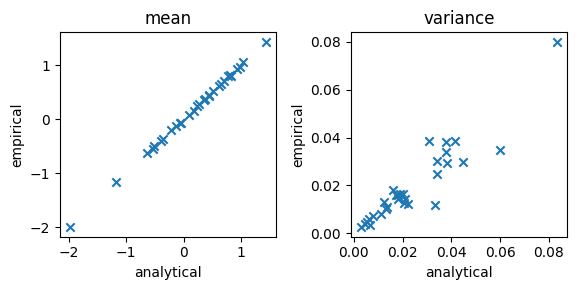
\includegraphics[width=0.6\columnwidth]{GP_neuron_sim.png}
    \caption{Empirical vs Analytical mean and variance values, repeated for different $\mu_x,\sigma_x^2$}
    \label{fig:GP_sim}
\end{figure}

\end{document}
